\begin{ledgroupsized}[r]{120mm}
 \footnotesize 
 \pstart 
 \noindent\textbf{\"{U}berlieferung:}
 \pend
 \end{ledgroupsized}

  
 \begin{ledgroupsized}[r]{114mm}
 \footnotesize 
 \pstart \parindent -6mm
 \makebox[6mm][l]{\textit{L}}Konzept: LH XXXVII 4 Bl. 34. Papierstreifen 23 x 6 cm, tlw. unregelm\"{a}{\ss}ig beschnitten. Bl. 34 r\textsuperscript{o} 8 \unitfrac{1}{2} Z., Bl. 34 v\textsuperscript{o} 1 \unitfrac{1}{2} Z. 1 Fig. auf Bl. 34 r\textsuperscript{o} unterhalb der 1. Z. rechts. Text umlaufend. \pend
 \end{ledgroupsized}
 %\normalsize
 \vspace*{5mm}
 \begin{ledgroup}
 \footnotesize 
 \pstart
\noindent\footnotesize{\textbf{Datierungsgr\"{u}nde}: Die Datierung erfolgt aufgrund des Wasserzeichens, das in mathematischen Manuskripten aus dem Fr\"{u}hjahr 1673 des \"{O}fteren (\textit{LSB} VII, 4 N. 15-17) nachgewiesen ist.}
 \pend
 \end{ledgroup}

 \vspace*{8mm}
 \pstart 
 \normalsize
\begin{wrapfigure}{l}{0.4\textwidth}
 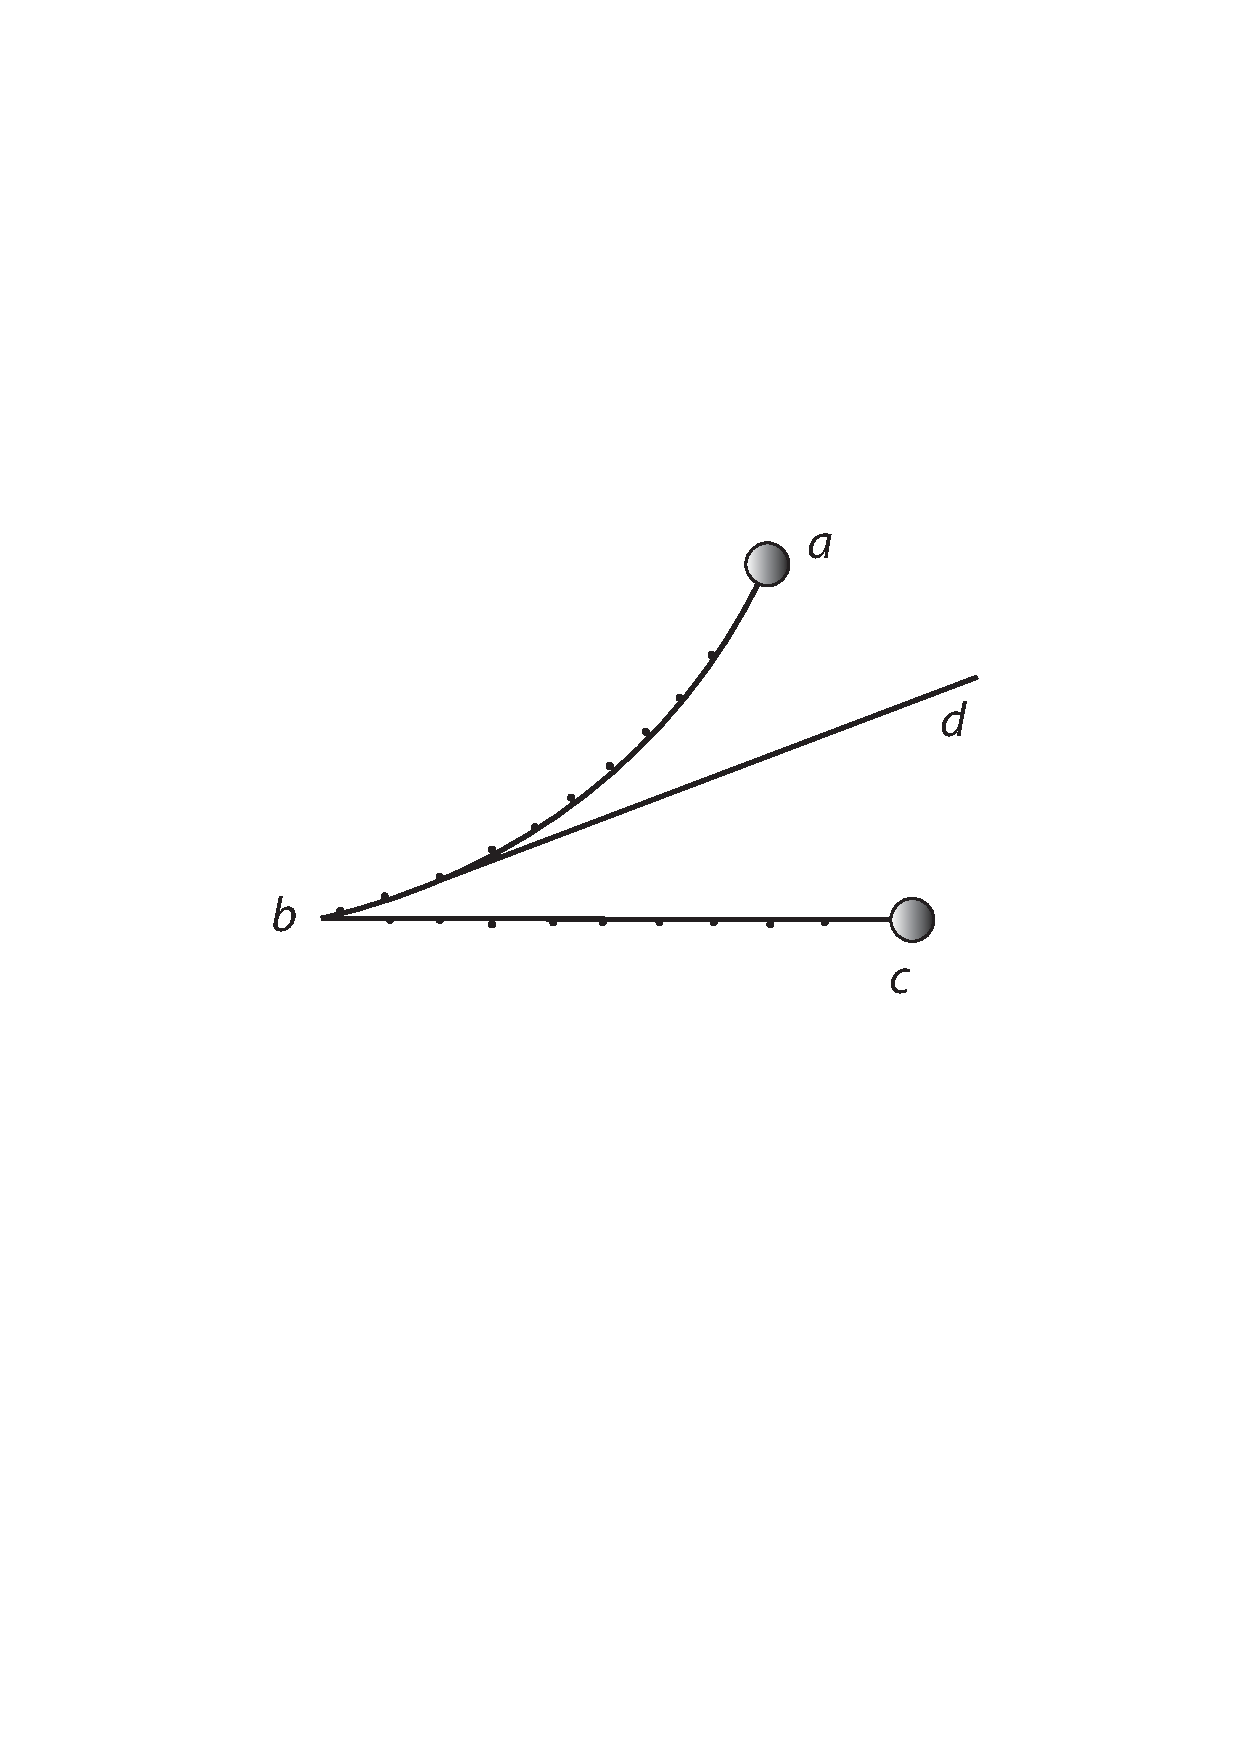
\includegraphics[width=0.4\textwidth]{images/lh374_34rkonvertiert.pdf}\\
\rule[0cm]{23mm}{0cm}\textit{Fig. 1}
%\caption{Fig. 1}
\end{wrapfigure}
[34~r\textsuperscript{o}] Experimentum notabile quo definiri possit, omniane in curvis peragantur per tangentes. Supponamus corpus aliquod linea quadam curva ferri, ut parabolica \textit{ab} aliudque in linea recta ei concurrere, quaeritur post momentum concursus\protect\index{Sachverzeichnis}{momentum concursus}, quaenam futura sit linea motus. Ducatur tangens \textit{bd} crediderit aliquis, cum directio curvae, in puncto \textit{b} sit in tangente \textit{db} aliaque accedat directio in recta \textit{cb} motum esse compositum ex his duabus directionibus. Sed hoc falsum est. Idem enim eveniret, si id verum esset, \edtext{ac}{\lemma{}\Afootnote{\textit{Links am Rand}: Imo non est absurdum.}} si corpus \textit{a} in linea recta \textit{bc} moveretur, quod est absurdum. Igitur sic potius cogitandum est, motum esse compositum \edtext{ex}{\lemma{compositum}\Bfootnote{ \textit{ (1) }\ in \textit{ (2) }\ ex \textit{ L}}} curvilineo illo et rectilineo, \edtext{aut potius}{\lemma{rectilineo,}\Bfootnote{ \textit{ (1) }\ quasi s \textit{ (2) }\ aut potius \textit{ L}}} ex tribus illis (pluribusve) directionibus, duabus nimirum (pluribusve) curvam constituentibus [34~v\textsuperscript{o}] et nova rectilinea accedente unde novum curvae genus vel forte prioris curvae nova species.\pend
 

